\item O disco circular de \SI{25}{\kilogram} é fixado ao garfo através de um eixo liso $A$. O parafuso $C$ é usado para travar o disco ao garfo. Se o garfo é submetido a um torque $M=(5t^{2})\,\SI{}{\newton\cdot\meter}$, onde $t$ é dado em segundos, e o disco está travado, determine a velocidade angular do garfo quando $t=\SI{3}{\second}$, partindo do repouso. Despreze a massa do garfo.

\import{../answers}{answer-6}

\vspace{-1cm}
\begin{flushright}
	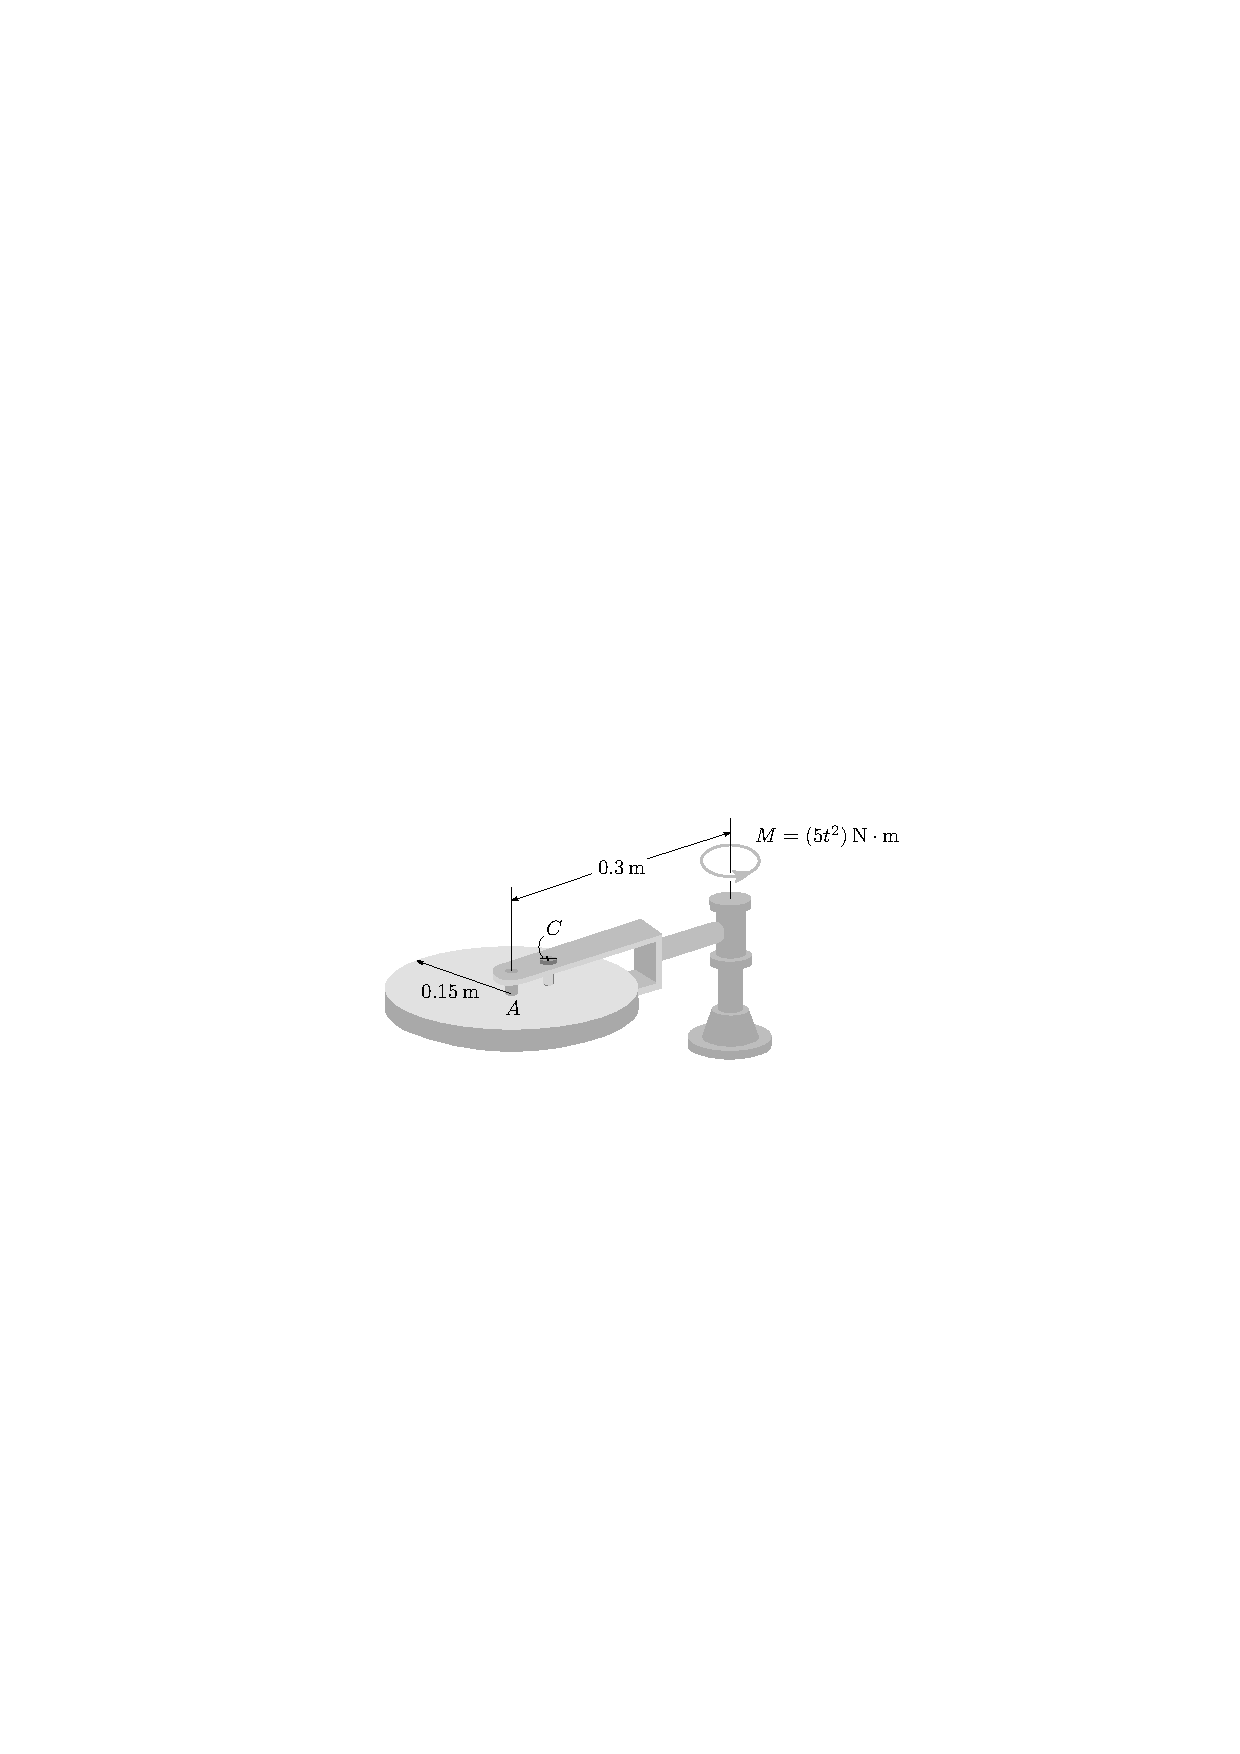
\includegraphics[scale=1.25]{../../images/draw_4_1}
\end{flushright}
